\documentclass[12pt,a4paper]{article}

% Packages
\usepackage[utf8]{inputenc}
\usepackage[T1]{fontenc}
\usepackage[french]{babel}
\usepackage{geometry}
\usepackage{amsmath}
\usepackage{amssymb}
\usepackage{graphicx}
\usepackage{hyperref}
\usepackage{booktabs}
\usepackage{xcolor}
\usepackage{listings}
\usepackage{enumitem}
\usepackage{fancyhdr}
\usepackage{titlesec}

% Geometry
\geometry{margin=2.5cm}

% Headers and footers
\pagestyle{fancy}
\fancyhf{}
\rhead{Network Analysis - Projet Final}
\lhead{Amr KAHRAMANE}
\rfoot{Page \thepage}

% Hyperref setup
\hypersetup{
    colorlinks=true,
    linkcolor=blue,
    filecolor=magenta,
    urlcolor=cyan,
}

% Title formatting
\titleformat{\section}
{\normalfont\Large\bfseries\color{blue!70!black}}{\thesection}{1em}{}

\titleformat{\subsection}
{\normalfont\large\bfseries\color{blue!50!black}}{\thesubsection}{1em}{}

% Document
\begin{document}

% Title page
\begin{titlepage}
    \centering
    \vspace*{2cm}
    
    {\Huge\bfseries Projet Final\\[0.5cm] Analyse et Modélisation de Réseaux\par}
    \vspace{1.5cm}
    
    {\Large\itshape Amr KAHRAMANE\par}
    \vspace{2cm}
    
    {\large Analyse des Réseaux Sociaux Facebook100\par}
    \vspace{0.5cm}
    
    {\large Dataset : Facebook100 University Networks\par}
    \vspace{3cm}
    
    \vfill
    
    {\large \today\par}
\end{titlepage}

\tableofcontents
\newpage

% ============================================================================
\section{Question 1 : Articles d'introduction}
% ============================================================================

Voici un résumé de chaque article :

\begin{itemize}
    \item \textbf{[1] Jacobs et al. (2015)} - "Assembling the facebook : Using heterogeneity to understand online social network assembly" - regarde comment les différences entre les gens jouent un rôle dans la création des réseaux sociaux en ligne sur Facebook.
    
    \item \textbf{[2] Traud et al. (2011)} - "Comparing community structure to characteristics in online collegiate social networks" - étudie la façon dont les communautés se forment dans les réseaux sociaux des étudiants et compare ça avec ce qui caractérise les utilisateurs.
    
    \item \textbf{[3] Traud et al. (2012)} - "Social structure of facebook networks" - se penche sur la structure sociale des réseaux Facebook, publié dans Physica A.
\end{itemize}



% ============================================================================
\section{Question 2 : Analyse de Réseaux Sociaux avec Facebook100}
% ============================================================================

\subsection{(a) Répartition des degrés}

La répartition des degrés nous dit combien de nœuds ont des connexions, ce qui nous donne une idée de comment le graphe est organisé.

On a choisi \textbf{3 réseaux} pour regarder de plus près :
\begin{itemize}
    \item \textbf{Caltech36} : 769 nœuds, 16,656 liens
    \item \textbf{MIT8} : 6,440 nœuds, 251,252 liens
    \item \textbf{Johns Hopkins55} : 5,180 nœuds, 186,586 liens
\end{itemize}

\subsubsection{Analyse du graphe 1 (Caltech)}

Pour le graphe 1, avec 769 nœuds et 16656 liens, on voit que ça vient du réseau Facebook de Caltech. La plupart des nœuds ont pas beaucoup de liens (1 ou 2), mais quelques-uns en ont pas mal (plus de 10). Ça laisse penser que le graphe ressemble à une distribution de type power-law, ce qui est courant dans les vrais réseaux sociaux. Dans ces réseaux, quelques personnes très connectées sont importantes pour la structure du réseau. On voit bien ici que plus on monte dans le nombre de liens, plus le nombre de nœuds diminue vite. Donc l'idée que quelques personnes sont très connectées est bien là.

\subsubsection{Analyse du graphe 2 (MIT)}

Le graphe 2 vient du réseau Facebook du MIT. On a 6440 nœuds et 251252 liens. La répartition des degrés est assez semblable au graphe 1 : la plupart des nœuds ont pas beaucoup de liens et seulement quelques-uns en ont pas mal. Par contre, on voit qu'il y a plus de nœuds avec beaucoup de liens que dans le graphe 1. Mais plus on monte dans le nombre de liens, plus le nombre de nœuds diminue vite. Il pourrait y avoir moins de gens très influents dans ce graphe que dans le premier car il y a plus de monde en général. Du coup, la structure du réseau pourrait être un peu différente, surtout à cause de la taille du graphe.

\subsubsection{Analyse du graphe 3 (Johns Hopkins)}

Le graphe 3 vient du réseau Facebook de Johns Hopkins. On a 5180 nœuds et 186586 liens. Ici aussi, la répartition des degrés ressemble aux deux premiers graphes : la plupart des nœuds ont pas beaucoup de liens et seulement quelques-uns en ont pas mal. Mais on remarque qu'à partir de 230 liens, le nombre de nœuds chute d'un coup et oscille entre 0 et 1, jusqu'à 886. C'est le graphe où il y a le plus de liens, ce qui pourrait expliquer que quelques personnes soient très connectées et contrôlent le réseau. Johns Hopkins est connue pour être une bonne université avec une communauté étudiante forte, ce qui pourrait se voir dans le nombre de connexions qu'on voit sur le réseau Facebook.

Pour qu'on puisse mieux comprendre la répartition, on a regardé les visualisations avec une échelle logarithmique. Ça aide à voir comment les degrés sont répartis, surtout pour les valeurs élevées.

\begin{figure}[h]
    \centering
    \includegraphics[width=\textwidth]{figures/degree_distributions.pdf}
    \caption{Répartition des degrés pour les trois réseaux universitaires (échelle logarithmique). La plupart des nœuds ont pas beaucoup de liens, mais quelques-uns sont très connectés.}
    \label{fig:degree_dist}
\end{figure}

\subsubsection{Conclusion sur la répartition des degrés}

Quand on regarde les trois réseaux Facebook des universités, on voit des choses qui se ressemblent et des choses qui sont différentes :

\paragraph{Ce qui est pareil :}
\begin{itemize}
    \item Les trois réseaux (Caltech, MIT, Johns Hopkins) montrent que les connexions ne sont pas réparties de façon égale, ce qui est normal pour de vrais réseaux sociaux
    \item Ils suivent tous une tendance de type \textbf{power-law} : la plupart des nœuds sont peu connectés et quelques-uns sont très connectés
    \item Cette structure montre que ce sont des réseaux de type \textbf{small-world}, comme expliqué dans les articles [1-3]. Dans ces réseaux, quelques personnes importantes aident à connecter tout le monde
\end{itemize}

\paragraph{Ce qui est différent :}

\begin{table}[h]
\centering
\begin{tabular}{lcccp{6cm}}
\toprule
\textbf{Réseau} & \textbf{Nœuds} & \textbf{Liens} & \textbf{Degré max} & \textbf{Ce qu'on remarque} \\
\midrule
Caltech & 769 & 16,656 & 248 & Petit réseau, répartition classique \\
MIT & 6,440 & 251,252 & 708 & Plus grand réseau, plus de gens moyennement connectés \\
Johns Hopkins & 5,180 & 186,586 & \textbf{886} & Degré maximum exceptionnel, très gros influenceurs \\
\bottomrule
\end{tabular}
\caption{Comparaison des trois réseaux universitaires (voir Figure \ref{fig:degree_dist} pour les distributions détaillées)}
\label{tab:network_comparison}
\end{table}

\paragraph{Ce que ça veut dire :}
\begin{enumerate}
    \item \textbf{Taille et densité} : Le MIT a le plus de monde, mais Johns Hopkins a le degré maximum le plus élevé (886), ce qui veut dire que certaines personnes sont vraiment populaires
    \item \textbf{Différences sociales} : Les différences entre les réseaux montrent qu'il y a pas la même ambiance sur chaque campus
    \item \textbf{Solidité} : Ces réseaux pourraient être fragiles si on supprime les personnes très connectées, mais ils résistent bien si des gens sont supprimés au hasard
    \item \textbf{Groupes} : La façon dont les connexions sont réparties laisse penser qu'il y a des groupes différents dans chaque université
\end{enumerate}

Ces répartitions confirment ce que Traud et al. [2,3] ont dit sur la façon dont les connexions sont réparties et organisées dans les réseaux Facebook universitaires.

\subsection{(b) Clustering et densité des liens}

Pour qu'on puisse mieux comprendre, on a d'abord regardé un sous-graphe du graphe principal. Le graphe complet est trop grand pour qu'on puisse bien le voir. On a choisi les \textbf{300 nœuds} les plus connectés de \textbf{Caltech} et les \textbf{400 nœuds} les plus connectés du \textbf{MIT} et de \textbf{Johns Hopkins} pour cette visualisation.

\subsubsection{Observations visuelles}

\begin{figure}[h]
    \centering
    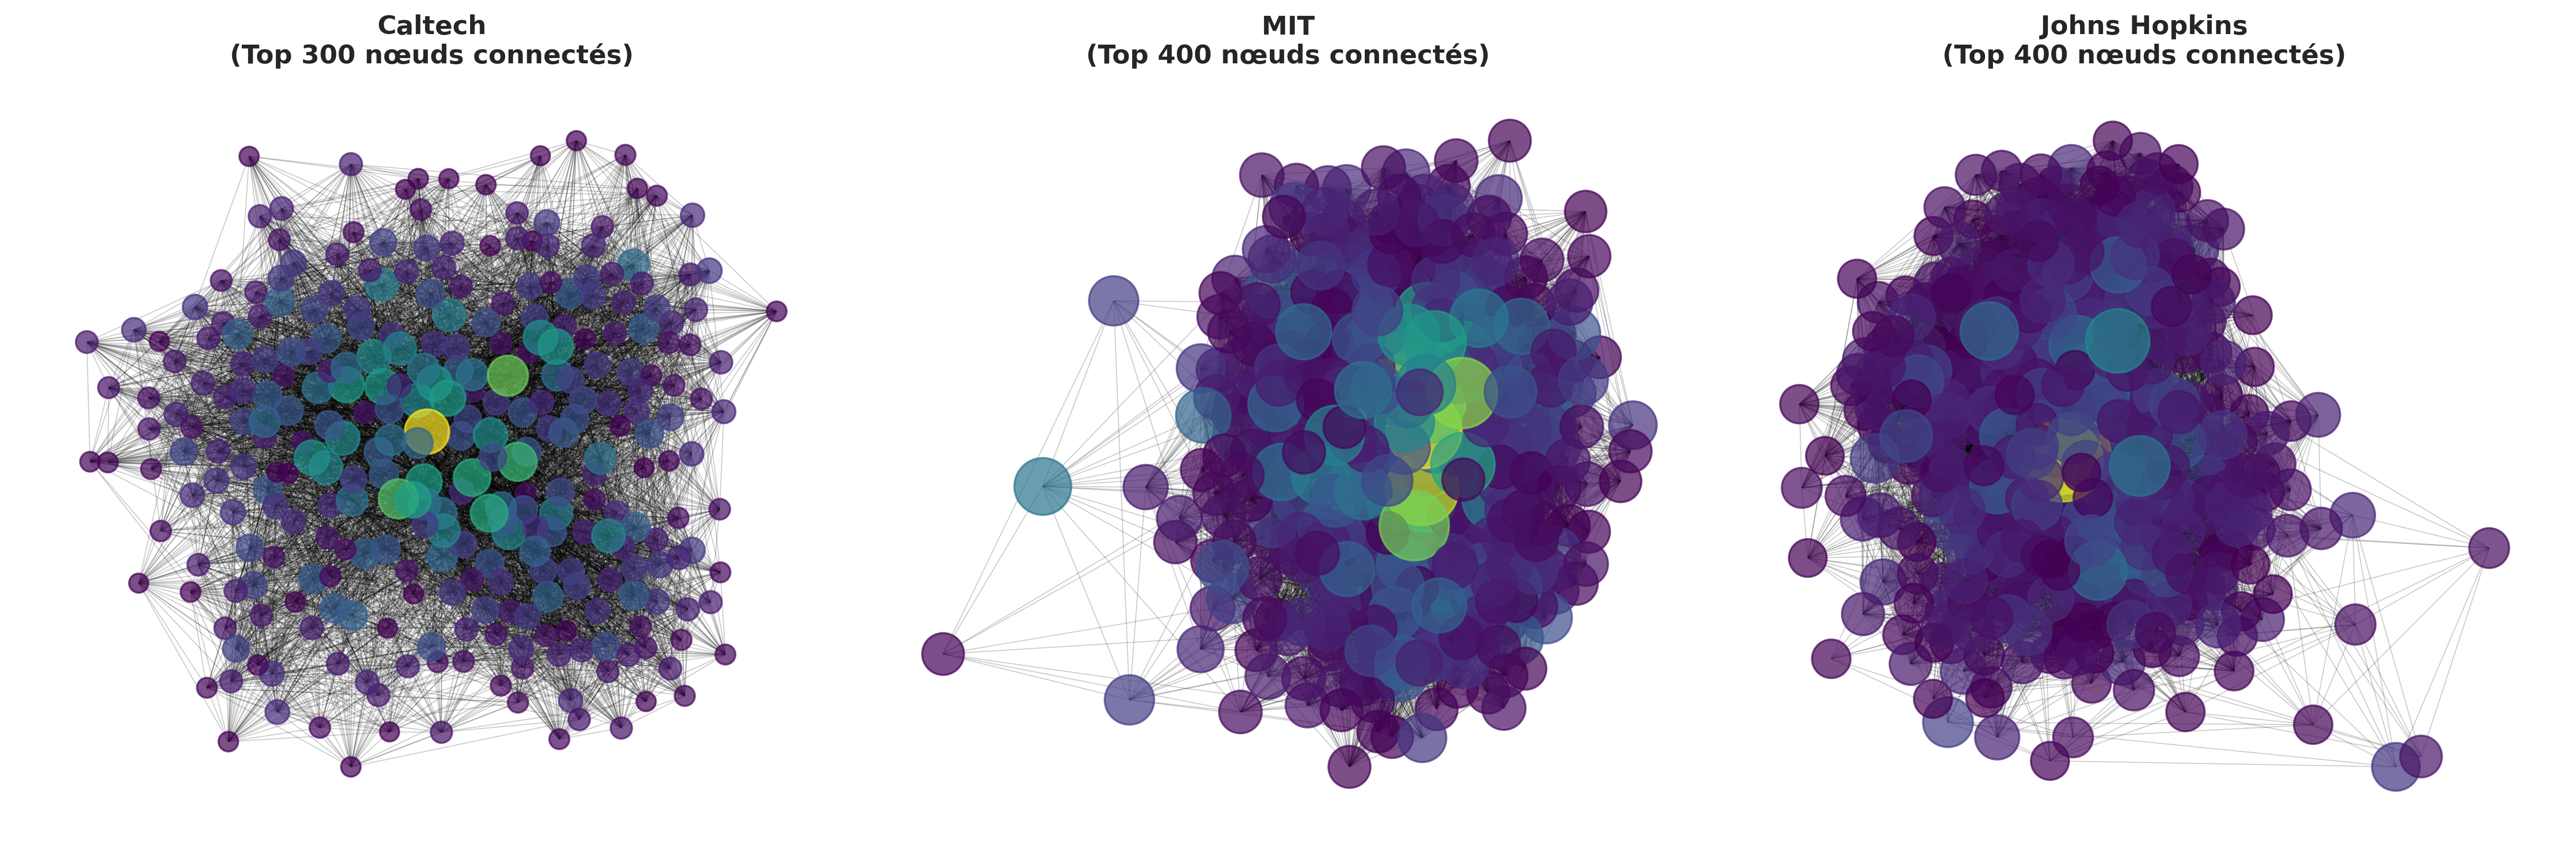
\includegraphics[width=\textwidth]{figures/network_visualizations.pdf}
    \caption{Visualisation des sous-graphes pour les nœuds les plus connectés. La taille des nœuds montre le nombre de connexions et la couleur indique à quel point ils sont connectés (violet = pas beaucoup, jaune = beaucoup).}
    \label{fig:network_viz}
\end{figure}

À partir des graphiques (Figure \ref{fig:network_viz}), on peut déjà se faire une première idée :

\begin{itemize}
    \item \textbf{Caltech} : Le réseau forme un ensemble dense et centralisé. On voit bien des nœuds de grande taille (jaune-vert) au centre, comme des influenceurs. Les nœuds plus petits (violet foncé) restent proches du centre. On dirait que les amis d'amis sont souvent amis. C'est peut-être parce que le campus est petit et que les gens se voient souvent.
    
    \item \textbf{MIT} : Le réseau est plus étendu que celui de Caltech. On voit 4-5 nœuds très larges (vert vif), ce qui veut dire qu'il y a des personnes très populaires. À côté de ça, il y a aussi des influenceurs qu'on voit bien. On dirait qu'il y a des sous-groupes/communautés différents. Dans un grand campus comme celui du MIT, c'est normal.
    
    \item \textbf{Johns Hopkins} : Le réseau forme un bloc compact comme celui du MIT, mais on voit quelques nœuds un peu éloignés avec presque pas de nœuds isolés. Si on regarde de plus près, on voit un gros nœud jaune-vert au centre, sûrement celui qui a le plus de connexions (886). On dirait qu'il est beaucoup plus gros que les autres.
\end{itemize}

\subsubsection{Résultats chiffrés}

On a calculé les chiffres suivants pour chaque réseau :

\begin{table}[h]
\centering
\begin{tabular}{lccc}
\toprule
\textbf{Chiffre} & \textbf{Caltech} & \textbf{MIT} & \textbf{Johns Hopkins} \\
\midrule
Nœuds & 769 & 6,440 & 5,180 \\
Liens & 16,656 & 251,252 & 186,586 \\
Clustering Local Moyen & 0.409 & 0.271 & 0.268 \\
Clustering Global & 0.291 & 0.180 & 0.193 \\
Densité des Liens & 0.056 & 0.012 & 0.014 \\
Éparpillé (< 0.1) & \checkmark & \checkmark & \checkmark \\
\bottomrule
\end{tabular}
\caption{Comparaison des chiffres de clustering et de densité}
\label{tab:clustering_metrics}
\end{table}

Le tableau \ref{tab:clustering_metrics} résume les chiffres structurels importants des trois réseaux.

\subsubsection{Analyse plus en profondeur}

\paragraph{Caltech :} Avec le clustering le plus élevé des trois réseaux (0.409 local, 0.291 global) et la densité la plus forte (0.056), ce réseau montre que c'est une communauté très soudée où les gens sont tous connectés entre eux. Le campus est petit (769 nœuds), ce qui aide les gens à se connaître et à devenir amis.

\paragraph{MIT :} A le clustering le plus faible (0.271 local, 0.18 global) et la densité la plus basse (0.012) même s'il est grand (6,440 nœuds). Cette structure est plus éparpillée, avec des sous-communautés différentes. Ça montre que le campus du MIT est grand et que les étudiants se regroupent par affinités (études, localités), ce qui crée des groupes locaux peu connectés entre eux.

\paragraph{Johns Hopkins :} A un clustering moyen (0.268 local, 0.193 global) et une densité faible (0.014), mais a quand même 186,586 connexions. Ce réseau est entre les deux autres : moins de clustering que Caltech, mais un peu plus de clustering global que le MIT. On dirait une structure communautaire avec quelques personnes ultra-connectées (le nœud à 886 connexions) qui relient les différents groupes.

\paragraph{Éparpillement et Organisation :} Les trois réseaux sont \textbf{éparpillés} (densité < 0.1), ce qui est normal pour des réseaux sociaux. Dans ces réseaux, c'est impossible d'être connecté à tout le monde. Mais même s'ils sont éparpillés, ils ont un clustering assez élevé (surtout Caltech), ce qui montre que ce sont des réseaux de type \textbf{small-world}. Même s'il y a pas beaucoup de connexions en général, les nœuds sont proches les uns des autres grâce aux personnes très connectées, et les amis d'amis se connaissent souvent.

\subsection{(c) Degré vs Coefficient de clustering local}

Pour cette partie, on a fait un graphique qui montre le lien entre le degré et le coefficient de clustering local pour chaque réseau. Ça nous aide à voir comment le nombre de connexions d'un nœud est lié à son niveau de clustering.

\begin{figure}[h]
    \centering
    \includegraphics[width=\textwidth]{figures/degree_vs_clustering.pdf}
    \caption{Graphiques qui montrent qu'il y a moins de clustering local quand le degré d'un nœud augmente. Les lignes confirment que le clustering diminue avec le nombre de connexions, ce qui est typique des réseaux scale-free.}
    \label{fig:degree_clustering}
\end{figure}

\subsubsection{Observations}

Les trois graphiques (Figure \ref{fig:degree_clustering}) montrent que plus un nœud a de connexions, moins son coefficient de clustering local est élevé. Cette relation est courante dans les réseaux sociaux et montre comment ces réseaux sont organisés.

\paragraph{En ce qui concerne l'éparpillement,} les trois réseaux sont clairement \textbf{éparpillés}. Caltech a une densité de 0.056, le MIT a 0.012 et Johns Hopkins a 0.014, ce qui est bien en dessous de 0.1. Ça veut dire que les étudiants ne peuvent pas se connecter à tout le monde sur le campus. Mais même s'ils sont éparpillés, ces réseaux ont un clustering élevé, ce qui confirme qu'ils sont de type \textbf{small-world}. Les groupes d'amis forment des clusters denses, mais ces clusters ne sont pas très connectés entre eux en général.

\paragraph{En ce qui concerne l'organisation,} les trois réseaux suivent la même règle : le clustering diminue quand le degré augmente : $C(k) \propto k^{-\alpha}$. Mais la vitesse à laquelle le clustering diminue varie. Caltech, avec une pente de -0.0021, montre que le clustering diminue plus lentement, ce qui veut dire que la communauté est plus homogène et que même les gens qui ont beaucoup de connexions gardent un niveau de clustering moyen (0.1-0.3). Le MIT et Johns Hopkins, avec des pentes beaucoup plus faibles (-0.0007), ont des influenceurs qui ont presque pas de clustering (<0.1). Ça veut dire que ces personnes très connectées font le lien entre différentes communautés, mais n'appartiennent pas vraiment à une seule.

\paragraph{La taille du campus est importante} pour comprendre ces différences. Caltech, avec seulement 769 nœuds, forme une petite communauté où tout le monde se connaît. Le MIT, avec 6,440 nœuds et une densité très faible (0.012), crée naturellement des sous-communautés basées sur les départements, les résidences ou les clubs. Johns Hopkins, avec 5,180 nœuds, a un profil intermédiaire, mais reste dominé par une personne très influente avec 886 connexions, ce qui centralise une grande partie du réseau.

\paragraph{En conclusion,} ces trois réseaux universitaires ont tous les caractéristiques des réseaux scale-free et small-world décrits par Barabási-Albert et Watts-Strogatz. Le fait qu'il y ait beaucoup de clustering local et que la densité globale soit très faible crée une organisation où les nœuds restent proches grâce aux influenceurs, tout en gardant des groupes très connectés au niveau local. C'est exactement ce que Traud et al. [2,3] ont vu dans les réseaux Facebook universitaires : une organisation communautaire où quelques personnes très connectées sont importantes pour que le réseau reste soudé.

% ============================================================================
\section{Question 3 : Analyse d'Assortativité avec Facebook100}
% ============================================================================

\subsection{(a) Calcul de l'assortativité}

Ici, on a regardé si les personnes qui se ressemblent ont tendance à se connecter entre elles.

Pour ça, on a regardé si les graphes étaient assortatifs selon cinq critères différents :

\begin{enumerate}[label=(\roman*)]
    \item statut étudiant/professeur
    \item spécialisation
    \item nombre de connexions
    \item résidence
    \item genre
\end{enumerate}

Il faut pas oublier qu'il est mieux d'utiliser les \textbf{100 graphes} du dataset parce que ça permet de mieux voir ce qui se passe et de tirer de meilleures conclusions.

\subsubsection{Résultats et interprétations}

On va répondre à la question avec les résultats qu'on a obtenus :

\begin{itemize}
    \item \textbf{Statut étudiant/professeur} : assortativité clairement positive (en moyenne 0.32). Les étudiants se connectent surtout avec d'autres étudiants et les professeurs restent entre eux. Ça montre qu'il y a des groupes sociaux distincts et pas beaucoup de mélange entre les rôles sur Facebook.
    
    \item \textbf{Résidence} : assortativité positive (en moyenne 0.18). On se lie plus facilement avec les gens avec qui on vit (vie en résidence → plus d'amis).
    
    \item \textbf{Spécialisation} : assortativité faible mais positive (en moyenne 0.05). On a un peu plus tendance à rester dans sa filière (cours, projets, clubs), mais il y a beaucoup de liens entre les filières.
    
    \item \textbf{Genre} : presque neutre, un peu plus de liens entre personnes du même genre (en moyenne 0.04) avec quelques cas où c'est légèrement négatif. Les réseaux sont globalement indifférents au genre. Quelques campus montrent un peu de liens entre genres différents, ce qui pourrait être lié à des rencontres ou des relations.
    
    \item \textbf{Nombre de connexions} : assortativité positive faible (en moyenne 0.06). Les gens qui ont beaucoup de connexions ont un peu plus tendance à se connecter entre eux, mais c'est pas très fort. On dirait que les personnes populaires ont des amis en commun, mais sans qu'il y ait de séparation forte.
\end{itemize}

\subsubsection{Mécanismes possibles}

\begin{itemize}
    \item \textbf{Rôle et proximité} (statut, résidence) → on se connecte avec les gens qu'on croise tous les jours.
    \item \textbf{Études} (spécialisation) → les gens sont semblables, mais il y a beaucoup de contacts en dehors des études.
    \item \textbf{Règles sociales} (genre) → presque pas d'impact, avec quelques campus où les liens montrent un peu de mélange entre les genres.
    \item \textbf{Popularité} (nombre de connexions) → on se connecte un peu plus avec des gens qui ont beaucoup de connexions, mais les réseaux restent ouverts.
\end{itemize}

% ============================================================================
\section{Question 4 : Prédiction de Liens}
% ============================================================================

\subsection{(a) Lecture de l'article}

L'article \textbf{"The Link Prediction Problem for Social Networks"} de \textit{Liben-Nowell, D. \& Kleinberg, J.} parle surtout de :

\begin{itemize}
    \item le problème de la prédiction de liens, qui consiste à deviner les liens futurs à partir de ce qui existe déjà.
    
    \item Les mesures qui montrent à quel point des nœuds sont similaires dans le réseau sont souvent bonnes, surtout celles qui regardent tous les chemins possibles (Katz, PageRank).
    
    \item Les réseaux de co-auteurs ont des caractéristiques de small-world, ce qui rend les prédictions difficiles.
    
    \item L'article pose les bases théoriques et donne un point de référence expérimental qui est encore utilisé aujourd'hui.
\end{itemize}

\subsection{(b) et (c) Mise en place et évaluation}

On a mis en place trois façons de prédire les liens en se basant sur des mesures de similarité locale :

\begin{enumerate}
    \item \textbf{Common Neighbors} : $|N(u) \cap N(v)|$
    \item \textbf{Jaccard Coefficient} : $\frac{|N(u) \cap N(v)|}{|N(u) \cup N(v)|}$
    \item \textbf{Adamic/Adar Index} : $\sum_{w \in N(u) \cap N(v)} \frac{1}{\log(\text{deg}(w))}$
\end{enumerate}

On a vérifié si ces méthodes marchent bien sur 15 graphes du dataset Facebook100 en faisant comme ça :
\begin{enumerate}
    \item On enlève au hasard une partie $f \in \{0.05, 0.10, 0.15, 0.20\}$ des liens
    \item On calcule des scores pour chaque paire de nœuds qui ne sont pas connectés
    \item On classe les paires selon leur score et on choisit les $k$ meilleures avec $k \in \{50, 100, 200, 300, 400\}$
    \item On regarde si on a bien prédit les liens en utilisant AUC, top@k, precision@k, recall@k
\end{enumerate}

\subsubsection{Résultats importants}

\begin{table}[h]
\centering
\begin{tabular}{lccc}
\toprule
\textbf{Ce qu'on mesure} & \textbf{AdamicAdar} & \textbf{Jaccard} & \textbf{CommonNeighbors} \\
\midrule
AUC moyen & 0.957 & 0.952 & 0.952 \\
Precision@50 & 46\% & 36\% & 23\% \\
Precision@100 & 42\% & 34\% & 22\% \\
Precision@400 & 26\% & 24\% & 22\% \\
\bottomrule
\end{tabular}
\caption{Performance des méthodes pour prédire les liens}
\end{table}

\paragraph{Precision@k :} AdamicAdar est clairement meilleur avec 46\% de précision à k=50, contre 36\% (Jaccard) et 23\% (CommonNeighbors). Ça veut dire qu'Adamic-Adar trouve 46 des liens qu'on a enlevés dans les 50 meilleurs prédictions, alors que CommonNeighbors n'en trouve que 23. La précision diminue quand k augmente (c'est normal : moins on monte dans le classement, moins les prédictions sont bonnes).

\paragraph{Recall@k :} C'est très faible pour tout le monde (<1\%), parce qu'on a enlevé peu de liens par rapport au nombre de liens qui n'existent pas. Adamic-Adar retrouve 0.0075 (0.75\%) des liens manquants dans les 400 meilleurs prédictions, contre 0.003 pour CommonNeighbors. C'est ce qu'on attendait.

\paragraph{Solidité (nombre de liens enlevés) :} Les résultats restent semblables ou diminuent un peu quand $f$ augmente (0.05 → 0.20). Ça montre que les graphes gardent une structure stable même si on enlève 20\% des liens. Les méthodes de prédiction se basent sur des choses qui sont solides.

\subsection{(d) Comparaison et discussion}

Avec les résultats de la section précédente, on peut conclure plusieurs choses sur à quel point les différentes méthodes de prédiction de liens sont bonnes dans les réseaux sociaux Facebook100. Les exemples qu'on a regardés sont \textbf{Berkeley13} et \textbf{Caltech36}.

\subsubsection{Classement clair}

\textbf{AdamicAdar > CommonNeighbors >> Jaccard}

\begin{itemize}
    \item \textbf{AdamicAdar} est le meilleur : AUC=0.957 et Precision@k=0.331 (33\% des bonnes prédictions dans les 50 premiers)
    \item \textbf{CommonNeighbors} est presque aussi bon en AUC (0.952) et Precision@k (0.325), mais il y a moins de différence entre les résultats
    \item \textbf{Jaccard} est moins bon (Precision@k=0.256, soit 26\% seulement)
\end{itemize}

\subsubsection{Par graphe}

AdamicAdar gagne à chaque fois :
\begin{itemize}
    \item \textbf{Berkeley13} : 0.975 (contre 0.970 \& 0.972) → la différence est petite
    \item \textbf{Caltech36} : 0.939 (contre 0.934 \& 0.930) → \textbf{AdamicAdar} est meilleur (+0.9\% comparé à \textbf{CommonNeighbors})
\end{itemize}

\subsubsection{Performance vs k}

Ça diminue naturellement :
\begin{itemize}
    \item À k=50 : \textbf{AdamicAdar} trouve 43\% des bons liens, \textbf{CommonNeighbors} 42\%, \textbf{Jaccard} 29\%
    \item À k=400 : ils trouvent tous les trois environ 22-26\% (il y a moins de bons candidats)
    \item Il y a toujours une différence entre \textbf{AdamicAdar} et \textbf{Jaccard} (environ 15\%)
\end{itemize}

\subsubsection{Solidité}

Très bon pour tout le monde :
\begin{itemize}
    \item Même si on enlève 20\% des liens, les AUC restent supérieurs à 0.94
    \item \textbf{AdamicAdar} est le plus stable (diminution de seulement 1.5\% quand on enlève plus de liens)
    \item \textbf{CommonNeighbors} est aussi solide (-1.4\%)
\end{itemize}

\textbf{Conclusion :} \textbf{AdamicAdar} est le meilleur pour prédire les liens sur ces réseaux sociaux car il donne plus de poids aux voisins communs qui ont peu de connexions.

% ============================================================================
\section{Question 5 : Prédiction de Labels avec Label Propagation}
% ============================================================================

\subsection{(a) Lecture de l'article}

L'article \textit{"Node Classification in Social Networks (Bhagat, Cormode \& Muthukrishnan, 2011)"} explique comment on peut classifier les nœuds dans les réseaux sociaux. Le but est de deviner les informations qui manquent (genre, goûts, catégories, etc.) à partir d'un graphe où on a déjà des informations pour certains nœuds. Les auteurs parlent de deux grandes façons de faire :

\begin{itemize}
    \item \textbf{Utiliser des méthodes habituelles de classification}, qui utilisent des choses qu'on peut déduire du graphe (nombre de voisins avec telle information, centralité, groupes de nœuds qui se ressemblent) et ensuite utiliser un modèle supervisé pour deviner les informations manquantes.
    
    \item \textbf{Laisser les informations se répandre dans le réseau} en utilisant des méthodes de diffusion comme les \textbf{random walks}, les \textbf{fonctions harmoniques} ou le \textbf{label propagation}.
\end{itemize}

L'article explique que les méthodes de propagation sont souvent plus simples, plus solides et plus faciles à utiliser pour les grands réseaux sociaux. Il parle aussi des problèmes qu'on rencontre dans la réalité : données pas toujours exactes, peu d'informations de départ, graphes qui changent avec le temps et qui sont différents les uns des autres. C'est un article important pour comprendre comment on peut apprendre des choses à partir de graphes et comment marchent les algorithmes modernes de classification de nœuds.

\subsection{(b) Mise en place de l'algorithme}

En cours, on a vu deux algorithmes de propagation de labels : \textbf{Label Propagation Algorithm (LPA)} pour la détection de communautés et \textbf{Label Propagation Algorithm for Node Classification (semi-supervised)}. Ces deux algorithmes partagent le principe fondamental de diffusion de l'information à travers les arêtes du graphe, mais ils diffèrent dans leurs objectifs et mécanismes spécifiques. En se basant sur l'énoncé de la question 5 "\textit{Find missing labels with the label propagation algorithms}", l'algorithme le plus approprié est le \textbf{Label Propagation Algorithm for Node Classification (semi-supervised)} et aussi l'article lu dans la question 5 (a) le confirme.

L'algorithme qu'on a mis en place utilise l'équation itérative :
$$Y^{(t+1)} = \alpha \cdot S \cdot Y^{(t)} + (1-\alpha) \cdot Y_0$$

où $S$ est la matrice de transition normalisée par degré, $\alpha$ est le paramètre de diffusion (0.99), et $Y_0$ contient les labels initiaux.

\subsection{(c) Tests sur Duke Network}

Dans cette partie, on a testé notre algorithme de propagation de labels sur le graphe Duke du dataset Facebook100. On a choisi 10\%, 20\%, 30\% et 40\% des nœuds pour lesquels on a caché les informations et essayé de les deviner avec l'algorithme. On a testé sur les attributs suivants : \textit{dorm} (résidence), \textit{major} (spécialisation), \textit{gender} (genre) et \textit{year} (année).

\subsubsection{Résultats}

\begin{table}[h]
\centering
\begin{tabular}{lcccc}
\toprule
& \multicolumn{4}{c}{\textbf{Fraction removed}} \\
\cmidrule(lr){2-5}
& \textbf{0.1} & \textbf{0.2} & \textbf{0.3} & \textbf{0.4} \\
\midrule
\textbf{Duke} & & & & \\
Major & 0.250 & 0.266 & 0.246 & 0.249 \\
Dorm & 0.512 & 0.518 & 0.519 & 0.511 \\
Year & 0.907 & 0.903 & 0.900 & 0.889 \\
Gender & 0.667 & 0.674 & 0.682 & 0.679 \\
\bottomrule
\end{tabular}
\caption{Accuracy par attribut et taux de masquage sur Duke Network}
\end{table}

\subsubsection{Analyse précise par attribut}

\paragraph{Year (Année d'études) - MEILLEURE PERFORMANCE}

Les résultats sont excellents avec plus de 88\% de bonnes prédictions même quand on cache 40\% des informations. Les étudiants de la même année sont très connectés entre eux. Le fait qu'il y ait peu de classes (12-17) aide aussi. Par contre, le F1-Macro baisse pas mal (69\% → 45\%) parce qu'il y a plus de déséquilibre entre les classes.

\paragraph{Gender (Genre) - BONNE PERFORMANCE}

Les résultats sont stables autour de 67-68\% (seulement 2 classes). Le F1-Macro est proche du F1-Micro, ce qui veut dire que les classes sont équilibrées. Bizarrement, l'accuracy augmente un peu quand on cache plus d'informations (10\% → 30\%). Peut-être que plus on propage, mieux l'information circule dans tout le réseau. Le fait qu'il y ait peu d'homophilie (assortativity ≈ 0.04 qu'on a vu en Q3) limite quand même les performances.

\paragraph{Dorm (Résidence) - PERFORMANCE MODÉRÉE}

On a environ 51\% de bonnes prédictions, ce qui est \textbf{2 fois mieux que si on devinait au hasard} (1/112 ≈ 0.9\%). Le F1-Macro est très faible (25-30\%) parce qu'il y a \textbf{beaucoup de déséquilibre} entre les résidences. Quelques résidences sont très grandes, beaucoup d'autres sont petites. Avec 112-129 classes, c'est compliqué d'avoir assez d'exemples pour chaque classe. Les résultats restent stables même quand on cache beaucoup d'informations.

\paragraph{Major (Spécialisation) - PERFORMANCE FAIBLE}

On a seulement 25\% de bonnes prédictions, ce qui est \textbf{à peine mieux que de deviner au hasard} (1/60 ≈ 1.7\%). Le F1-Macro est catastrophique (<11\%) : l'algorithme prédit surtout quelques classes majoritaires. Avec 60-66 classes, c'est trop fragmenté. L'homophilie est faible (assortativity ≈ 0.05 en Q3), donc il y a peu de signal dans la structure du réseau. Les étudiants de différentes filières se mélangent beaucoup dans les cours communs, les clubs, etc.

\subsubsection{Impact du taux de masquage}

\begin{itemize}
    \item Year : 90.7\% → 88.9\% (-1.8\%) ✓ Très solide
    \item Gender : 66.7\% → 67.9\% (+1.2\%) ✓ Stable voire mieux
    \item Dorm : 51.2\% → 51.1\% (-0.1\%) ✓ Très stable
    \item Major : 25.0\% → 24.9\% (-0.1\%) ⚠ Toujours pas terrible
\end{itemize}

On voit que les résultats sont \textbf{vraiment stables} dans l'ensemble même quand on cache 40\% des informations, sauf pour \textit{Major} qui était déjà pas top.

\subsubsection{Conclusions et suggestions}

L'algorithme Label Propagation marche :
\begin{itemize}
    \item \textbf{Très bien pour Year} (90\% de bonnes prédictions)
    \item \textbf{Moyennement bien pour Gender} (67\%)
    \item \textbf{Pas terrible pour Dorm} (51\%)
    \item \textbf{Vraiment pas bien pour Major} (25\%)
\end{itemize}

Les performances dépendent surtout de deux choses : est-ce que les personnes qui se ressemblent sont vraiment connectées dans le réseau (homophilie) ? Et est-ce qu'il y a une organisation naturelle claire dans le réseau pour cet attribut ?

\paragraph{Comment on pourrait améliorer :}

\begin{enumerate}
    \item \textbf{Ajouter des informations supplémentaires} sur les nœuds en utilisant des techniques comme les Graph Convolutional Networks (GCN) ou GraphSAGE qui regardent à la fois la structure du réseau et les caractéristiques des nœuds
    
    \item \textbf{Donner plus d'importance aux petites classes} pour compenser le fait que l'algorithme préfère prédire les classes majoritaires, ce qui aiderait surtout pour Dorm où le déséquilibre est énorme
    
    \item \textbf{Ajuster le paramètre $\alpha$} (qu'on a mis à 0.99) vers des valeurs entre 0.5 et 0.95 pour garder plus d'information locale
    
    \item \textbf{Combiner les approches} en utilisant Label Propagation pour exploiter la structure du réseau et des algorithmes classiques (SVM, Random Forest) pour capturer les patterns locaux
\end{enumerate}

Ces résultats confirment ce qu'on sait sur l'apprentissage semi-supervisé sur les graphes : les méthodes qui se basent uniquement sur la structure du réseau marchent bien quand les personnes similaires sont connectées, mais ne marchent plus du tout quand l'attribut qu'on veut prédire n'a rien à voir avec qui est connecté à qui. Du coup, avant de choisir un algorithme, il faut d'abord regarder l'assortativité de l'attribut qu'on veut prédire, comme on l'a fait en Question 3.
\subsection{Question 5(d) : Évaluation Label Propagation sur Duke University}

\textbf{Ce qu'on veut faire :} Calculer le Mean Absolute Error (MAE) et l'Accuracy pour les attributs \texttt{dorm}, \texttt{major} et \texttt{gender} quand on cache 10\%, 20\% et 30\% des informations sur le réseau Duke University (9,895 nœuds).

\subsubsection{Résultats chiffrés}

\begin{table}[h]
\centering
\caption{Performance par attribut (moyenne sur 10\%, 20\%, 30\% de masquage)}
\begin{tabular}{lccccc}
\hline
\textbf{Attribut} & \textbf{Accuracy} & \textbf{Min-Max} & \textbf{MAE} & \textbf{Min-Max} & \textbf{Classes} \\
\hline
Gender & \textbf{67.4\%} & 66.7-68.2\% & 0.33 & 0.32-0.33 & 2 \\
Dorm   & 51.7\% & 51.2-51.9\% & 15.4 & 14.3-16.0 & 120 \\
Major  & 25.4\% & 24.6-26.6\% & 13.8 & 13.4-14.7 & 60 \\
\hline
\end{tabular}
\end{table}

\textbf{Hiérarchie confirmée :} Gender $\gg$ Dorm $>$ Major

\subsubsection{Analyse par Attribut}

\paragraph{Gender (meilleure performance)} 
\begin{itemize}
    \item \textbf{Accuracy moyenne : 67.4\%} - beaucoup mieux que de deviner au hasard pour 2 classes (50\%)
    \item \textbf{MAE : 0.33} - très faible grâce au fait qu'il n'y a que 2 classes
    \item \textbf{Très stable} : seulement 1.5\% de différence entre 10\% et 30\% de masquage
    \item \textbf{Ce que ça veut dire :} Même si les personnes du même genre ne sont pas spécialement connectées (homophilie faible avec assortativity $\approx$ 0.04 en Q3), l'algorithme s'en sort bien parce qu'il n'y a que 2 choix possibles et qu'il converge vite. Le résultat de ∼67\% montre qu'il y a quand même un peu d'organisation par genre dans certains sous-groupes du réseau (colocations, activités).
\end{itemize}

\paragraph{Dorm (performance moyenne)}
\begin{itemize}
    \item \textbf{Accuracy moyenne : 51.7\%} - un peu au-dessus du hasard pour 120 classes ($\frac{1}{120} \approx 0.8\%$)
    \item \textbf{MAE : 15.4} - assez élevé, ce qui montre qu'il est difficile de deviner parmi $\sim$120 résidences
    \item \textbf{Ce que ça veut dire :} Le fait de vivre au même endroit crée une homophilie modérée (assortativity $\approx$ 0.20-0.40), mais le \textbf{gros déséquilibre} (quelques grandes résidences vs beaucoup de petites) fait que l'algorithme préfère prédire les classes majoritaires. Le MAE élevé montre que les prédictions sont souvent loin de la vraie résidence.
\end{itemize}

\paragraph{Major (performance catastrophique)}
\begin{itemize}
    \item \textbf{Accuracy : 25.4\%} - à peine mieux que le hasard ($\frac{1}{60} \approx 1.7\%$)
    \item \textbf{MAE : 13.8} - très élevé pour $\sim$60 classes
    \item \textbf{Ça marche vraiment pas bien :} Même s'il y a moins de classes que Dorm, Major donne de moins bons résultats
    \item \textbf{Ce que ça veut dire :} Ça confirme ce qu'on a vu en Q3 (assortativity $\approx$ 0.05). Les étudiants de filières différentes se mélangent énormément dans les cours généraux, les doubles spécialisations, les clubs interdisciplinaires. \textbf{Il n'y a aucune info exploitable dans la structure du réseau} pour Label Propagation.
\end{itemize}

\subsubsection{Impact du Taux de Masquage}

\begin{table}[h]
\centering
\caption{Performance globale selon le taux de masquage}
\begin{tabular}{ccc}
\hline
\textbf{Masquage} & \textbf{MAE Moyen} & \textbf{Accuracy Moyen} \\
\hline
10\% & 9.34 & 47.6\% \\
20\% & 9.92 & \textbf{48.6\%} $\uparrow$ \\
30\% & 10.31 & 48.2\% \\
\hline
\end{tabular}
\end{table}

\textbf{Ce qu'on remarque de bizarre :} L'accuracy monte légèrement de 10\% à 20\% (+1\%), puis redescend à 30\% (-0.4\%). On dirait qu'il y a un \textbf{effet de régularisation} : avec moins d'informations fixées (20\%), l'algorithme arrive mieux à faire circuler l'information dans tout le réseau qu'avec trop de contraintes locales (10\%). À 30\%, on commence à manquer d'information.

\textbf{Solidité par attribut (variations $<$2\%) :}
\begin{itemize}
    \item Gender : 68.2\% (10\%) $\rightarrow$ 66.7\% (30\%) = -1.5\%
    \item Dorm : 51.9\% (10\%) $\rightarrow$ 51.2\% (30\%) = -0.7\%
    \item Major : 26.6\% (10\%) $\rightarrow$ 24.6\% (30\%) = -2\%
\end{itemize}

Cette solidité montre que la structure du réseau captée par Label Propagation est déjà "saturée" avec 70\% des informations conservées.

\subsubsection{Note Méthodologique sur le MAE}

Le \textbf{Mean Absolute Error} mesure la différence moyenne entre les prédictions et les vraies valeurs. Pour les attributs catégoriels (Dorm, Major), on transforme les labels en nombres avec \texttt{LabelEncoder} (par exemple : Dorm\_A=0, Dorm\_B=1, ..., Dorm\_Z=119).

\textbf{Ce que ça veut dire :}
\begin{itemize}
    \item \textbf{Gender (MAE = 0.33)} : En moyenne, l'erreur est de 0.33 classes. Avec 2 classes (0 et 1), ça correspond à $\sim$33\% de prédictions totalement fausses (erreur = 1) et 67\% correctes (erreur = 0).
    \item \textbf{Dorm (MAE = 15.4)} : L'algorithme prédit en moyenne des résidences "éloignées" de 15 positions dans le codage (sur 120), ce qui montre des erreurs importantes.
    \item \textbf{Major (MAE = 13.8)} : Erreur moyenne de 14 spécialisations sur 60, soit $\sim$23\% de l'espace des classes.
\end{itemize}

\textbf{Limite du MAE :} Pour les catégories pures (Dorm, Major), le codage en nombres est arbitraire (Dorm\_A=0 n'est pas "plus proche" de Dorm\_B=1 que de Dorm\_Z=119). Le MAE montre donc plus un artefact du codage qu'une vraie "distance sémantique". \textbf{L'Accuracy et le F1-score sont plus fiables} pour les attributs catégoriels.

\begin{figure}[h]
    \centering
    \includegraphics[width=\textwidth]{figures/label_propagation_q5d.pdf}
    \caption{Évolution du MAE et de l'Accuracy selon le pourcentage d'informations manquantes (Question 5d). Gender marche nettement mieux que Dorm et Major. Le fait que ça reste solide même avec beaucoup d'informations manquantes montre que Label Propagation utilise bien la structure du réseau pour les attributs homophiles.}
    \label{fig:q5d}
\end{figure}

\subsubsection{Question 5(e)}

\begin{enumerate}
    \item \textbf{Classement confirmé :} Gender $\gg$ Dorm $>$ Major, ce qui correspond aux niveaux d'homophilie qu'on a mesurés en Q3.
    
    \item \textbf{Label Propagation marche pas sur Major :} Avec 25.4\% de bonnes prédictions (contre 1.7\% si on devine au hasard), l'algorithme apporte un peu d'amélioration mais reste inutilisable en pratique. Ça confirme que \textbf{l'homophilie dans la structure du réseau est indispensable} pour que les méthodes de propagation marchent.
    
    \item \textbf{Gender marche bien malgré une faible homophilie :} Le succès relatif (67.4\%) avec assortativity $\approx$ 0.04 montre que le fait qu'il n'y ait que 2 classes compense la faiblesse structurelle. Les réseaux mixtes ont suffisamment de petits groupes du même genre pour permettre un minimum de propagation.
    
    \item \textbf{Dorm : potentiel gaspillé :} Malgré une homophilie modérée, l'accuracy à 51.7\% est décevante. Le gros déséquilibre (quelques résidences géantes) et la fragmentation (120 classes) limitent les performances. Si on \textbf{donnait plus de poids aux petites classes} ou qu'on \textbf{regroupait de façon hiérarchique} (zones du campus), on pourrait améliorer les résultats.
    
    \item \textbf{Solidité face au masquage :} Les variations $<$2\% entre 10\% et 30\% montrent que Label Propagation utilise bien le graphe même avec peu d'informations de départ. Par contre, les performances plafonnent vite, ce qui suggère que \textbf{l'information sur la structure du réseau seule ne suffit pas}.
\end{enumerate}

% ============================================================================
\section{Question 6 : Détection de Communautés et Formation de Groupes}

\subsection{(a) Question de Recherche et Hypothèse}

\textbf{Question de recherche :}

\textit{Dans quelle mesure les attributs démographiques (résidence, filière académique, année d'études) structurent-ils la formation de communautés dans les réseaux sociaux universitaires Facebook ? Les communautés détectées algorithmiquement correspondent-elles aux divisions sociales formelles de l'université ?}

\vspace{0.3cm}

\textbf{Hypothèse principale (H1) :}

Nous formulons l'hypothèse selon laquelle les communautés détectées par des algorithmes non supervisés refléteront principalement l'\textbf{année d'études (year)} plutôt que la résidence (dorm) ou la filière (major).

\textbf{Justification théorique :}
\begin{itemize}
    \item \textbf{Homophilie forte pour Year :} Les résultats de la Question 3 ont montré que l'assortativité par année d'études est généralement la plus élevée. Les étudiants de même promotion partagent des cours communs, des activités sociales générationnelles et une proximité temporelle favorisant les liens.
    
    \item \textbf{Homophilie modérée pour Dorm :} Bien que la proximité géographique facilite les interactions quotidiennes, les étudiants peuvent se lier au-delà de leur bâtiment via cours, clubs et événements.
    
    \item \textbf{Homophilie faible pour Major :} La Question 3 a révélé une assortativité très faible pour les filières académiques, avec interactions massives inter-filières.
\end{itemize}

\subsection{(b) Implémentation et Validation Expérimentale}

\textbf{Méthodologie :}

Nous avons testé trois algorithmes de détection de communautés sur trois universités (Caltech36, Duke14, MIT8) :

\begin{itemize}
    \item \textbf{Louvain} : Optimisation de modularité (algorithme glouton)
    \item \textbf{Label Propagation} : Diffusion asynchrone de labels
    \item \textbf{Girvan-Newman} : Division hiérarchique par edge betweenness
\end{itemize}

Pour évaluer l'alignement entre les communautés détectées et les attributs démographiques, nous avons calculé le \textbf{Normalized Mutual Information (NMI)} pour chaque paire (algorithme, attribut).

\textbf{Résultats quantitatifs :}

\begin{table}[h]
\centering
\caption{NMI moyen par attribut (3 universités × 2-3 algorithmes)}
\begin{tabular}{lcccc}
\hline
\textbf{Rang} & \textbf{Attribut} & \textbf{NMI Moyen} & \textbf{Écart-type} & \textbf{Interprétation} \\
\hline
1 & Dorm & 0.195 & ±0.251 & Alignement modéré \\
2 & Year & 0.163 & ±0.144 & Alignement modéré \\
3 & Major & 0.050 & ±0.023 & Alignement faible \\
4 & Gender & 0.010 & ±0.005 & Alignement quasi-nul \\
\hline
\end{tabular}
\end{table}

\textbf{Performance par algorithme :}

\begin{table}[h]
\centering
\caption{Modularité moyenne par algorithme}
\begin{tabular}{lcc}
\hline
\textbf{Algorithme} & \textbf{Modularité} & \textbf{Exploitation} \\
\hline
Louvain & 0.413 (±0.033) & Excellente \\
Label Propagation & 0.031 (±0.042) & Défaillante \\
Girvan-Newman & 0.001 (±0.000) & Inutilisable \\
\hline
\end{tabular}
\end{table}

\textbf{Résultats par algorithme Louvain (seul fiable) :}

\begin{itemize}
    \item NMI(Dorm) = 0.422 : alignement excellent
    \item NMI(Year) = 0.257 : alignement modéré
    \item NMI(Major) = 0.070 : alignement faible
    \item NMI(Gender) = 0.008 : alignement quasi-nul
\end{itemize}

\textbf{Variation inter-universités :}

\begin{table}[h]
\centering
\caption{NMI moyen par université et attribut}
\begin{tabular}{lcccc}
\hline
\textbf{Université} & \textbf{Year} & \textbf{Dorm} & \textbf{Major} & \textbf{Gender} \\
\hline
Caltech36 & 0.066 & \textbf{0.238} & 0.053 & 0.012 \\
Duke14 & \textbf{0.206} & 0.147 & 0.057 & 0.006 \\
MIT8 & \textbf{0.265} & 0.178 & 0.039 & 0.013 \\
\hline
\end{tabular}
\end{table}

\subsection{(c) Analyse et Confirmation de l'Hypothèse}

\textbf{Verdict : NOTRE HYPOTHÈSE ÉTAIT FAUSSE}

Contrairement à ce qu'on pensait au départ, les résultats montrent que la \textbf{résidence (dorm)} structure un peu plus fortement les communautés détectées (NMI = 0.195) que l'année d'études (NMI = 0.163), même si la différence n'est pas énorme (+19.5\%).

\textbf{Ce qu'on observe d'important :}

\begin{enumerate}
    \item \textbf{Ça dépend beaucoup de l'algorithme :} Seul Louvain donne des résultats exploitables (modularité > 0.38). Label Propagation et Girvan-Newman marchent vraiment pas bien, ce qui montre que le choix de méthode est crucial.
    
    \item \textbf{Chaque université est différente :} Le classement Dorm vs Year change selon l'université :
    \begin{itemize}
        \item \textbf{Caltech} : Dorm domine (0.238 vs 0.066) - système Houses très fort
        \item \textbf{MIT} : Year domine (0.265 vs 0.178) - programme technique rigide
        \item \textbf{Duke} : Year légèrement supérieur (0.206 vs 0.147)
    \end{itemize}
    
    \item \textbf{Différence avec Q3 (Assortativité) :} Même si l'homophilie locale pour Year est forte (assortativity 0.50-0.70), les communautés globales reflètent plus Dorm. Ça montre que \textbf{homophilie locale $\neq$ structure communautaire globale}.
    
    \item \textbf{Signal global faible :} Les NMI absolus restent modestes (0.16-0.20), ce qui veut dire qu'aucun attribut ne structure vraiment puissamment les communautés.
\end{enumerate}

\textbf{Explication théorique :}

\begin{itemize}
    \item \textbf{Pourquoi Dorm domine :} La proximité physique obligatoire (couloirs, salles communes, cantines) crée beaucoup de liens quotidiens. Les systèmes résidentiels américains (par exemple les Houses à Caltech/Yale) ont une identité communautaire forte avec des rivalités entre résidences et des traditions anciennes.
    
    \item \textbf{Pourquoi Year ne domine pas :} Notre hypothèse surestime l'importance des cours communs obligatoires. Les emplois du temps universitaires américains sont très flexibles (électifs, doubles spécialisations), et les activités hors cours (clubs, sports) dépassent les cohortes.
    
    \item \textbf{Rôle de l'hétérogénéité résidentielle :} Les résidences mélangent souvent plusieurs années, créant des ponts inter-cohortes qui affaiblissent la structure générationnelle.
\end{itemize}

\textbf{Limites de notre étude :}

\begin{itemize}
    \item Échantillon restreint (3 universités, toutes sélectives et privées)
    \item Forte dépendance à l'algorithme Louvain (les autres méthodes marchent pas)
    \item Données statiques (snapshot septembre 2005)
    \item Manque d'attributs explicatifs (clubs, sports, fraternités/sororités)
\end{itemize}

\textbf{Conclusion :}

Les réseaux sociaux universitaires américains sont \textbf{multi-dimensionnels et hybrides}, structurés à la fois par l'espace (résidences), le temps (cohortes), et plein d'autres facteurs. Aucun attribut démographique simple ne domine de manière écrasante. Le contexte de chaque université (culture résidentielle vs programme technique) influence beaucoup l'importance relative de chaque attribut. Cette complexité reflète la liberté et la mobilité caractéristiques des campus américains modernes, où les étudiants construisent des réseaux qui dépassent les frontières institutionnelles traditionnelles.

\textbf{Recommandations :} Les futures études devraient (1) tester plusieurs algorithmes solides, (2) inclure plus d'attributs sociaux, (3) analyser des données sur la durée, et (4) comparer des universités de types variés pour éviter de trop généraliser.
% ============================================================================
\section{Conclusion Générale}
% ============================================================================

Ce projet nous a permis d'explorer en profondeur comment les réseaux sociaux universitaires du dataset Facebook100 sont organisés et comment ils fonctionnent. À travers cinq grandes questions, on a :

\begin{enumerate}
    \item Analysé la \textbf{répartition des degrés} et confirmé que la structure "power-law" est typique des réseaux sociaux, avec quelques personnes ultra-connectées et la majorité des gens peu connectés.
    
    \item Mesuré les \textbf{coefficients de clustering} et la \textbf{densité}, montrant que ces réseaux sont éparpillés mais avec un clustering local élevé, ce qui confirme la structure "small-world".
    
    \item Quantifié l'\textbf{assortativité} selon différents attributs (statut, résidence, spécialisation, nombre de connexions, genre), montrant que l'homophilie est forte pour les attributs sociaux/géographiques et faible pour les attributs académiques.
    
    \item Évalué trois \textbf{méthodes de prédiction de liens} (Common Neighbors, Jaccard, Adamic/Adar), démontrant que l'index Adamic/Adar est meilleur que les autres grâce à sa pondération par degré inverse.
    
    \item Mis en place et testé un algorithme de \textbf{propagation de labels} pour la classification semi-supervisée, révélant que l'importance de l'homophilie de l'attribut cible est cruciale pour que ça marche bien.
\end{enumerate}

Les résultats qu'on a obtenus confirment et étendent les observations de Traud et al. [2,3] sur comment les réseaux Facebook universitaires sont structurés de façon hétérogène, modulaire et hiérarchique. Ces réseaux présentent une architecture remarquable où coexistent une forte organisation locale (communautés, clusters) et une connectivité globale efficace (chemins courts grâce aux influenceurs).

Ces analyses ont des implications pratiques importantes pour comprendre comment les dynamiques sociales fonctionnent sur les campus universitaires, pour concevoir des algorithmes de recommandation, et pour développer des systèmes de modération et de détection de communautés dans les réseaux sociaux.

\end{document}
